\documentclass[10pt]{article}
\usepackage[italian]{babel}
\usepackage{array}
\usepackage{graphicx}
\usepackage[export]{adjustbox}
\usepackage{ragged2e}
\usepackage{float}
\usepackage[hidelinks]{hyperref}
\usepackage{caption}
\usepackage{listings}
\usepackage{xcolor}
\lstset{
  language=Java,
  basicstyle=\ttfamily\small,
  keywordstyle=\color{blue},
  commentstyle=\color{gray},
  stringstyle=\color{red},
  numbers=left,
  numberstyle=\tiny,
  breaklines=true,
  breakatwhitespace=true,
  showstringspaces=false,
  backgroundcolor=\color{white},
  frame=single
}

\setlocalecaption{italian}{contents}{Indice}

\begin{document}

\par\medskip
\begin{center}

\includegraphics[scale=0.1,center]{unifilogo/firenze2}
\end{center}

\begin{center}
\par\medskip
\textsc{{\large Università degli studi di Firenze}}\\
\par\medskip
\textsc{{\normalsize Dipartimento di Ingegneria Informatica}}\\
\par\medskip
\par\medskip
\hrule width 12cm height 1pt \par
\par\medskip
\par\medskip
\par\medskip
{\Huge \textbf{Apartament}}\\
\par\medskip
\par\medskip
\par\medskip
\hrule width 12cm height 1pt \par
\par\medskip
\par\medskip
{\Large \textbf{Link Github: \href{https://github.com/Pennelli02/SweProject}{https://github.com/Pennelli02/SweProject}}}
\par\medskip
\par\medskip
\hrule width 12cm height 1pt \par
\par\medskip
\par\medskip
\par\medskip
\emph{Autori:} \hfill \emph{Docente corso:}\\
\par\medskip
Pennelli Lorenzo Maria \hfill Vicario Enrico\\
\begin{FlushLeft}
Leuter Lorenzo\\
\end{FlushLeft}

\end{center}

\newpage

\tableofcontents

\newpage

\section{Introduzione}

\subsection{Descrizione del progetto}

L'obiettivo è creare un'applicazione java che permetta di gestire le prenotazioni di alloggi, in particolare verranno trattati B\&B, appartamenti e hotel. Gli utenti avranno la possibilità di effettuare ricerche e prenotazioni degli alloggi disponibili, selezionare il numero di persone che soggiorneranno, la data di inizio e di fine del soggiorno, e molti altri filtri che verranno spiegati successivamente. Inoltre, l'utente potrà anche cancellare le prenotazioni, inserire tra i preferiti gli alloggi e lasciare delle recensioni a essi. \`E inoltre presente un Admin che può cancellare definitivamente gli utenti,  gli alloggi o le recensioni, aggiungere nuovi alloggi e modificare gli alloggi già presenti.

\subsection{Architettura del progetto e Ambiente di sviluppo}

L'architettura del progetto è rappresentata dalla figura sottostante: 
\begin{center}
\hspace*{-1cm}
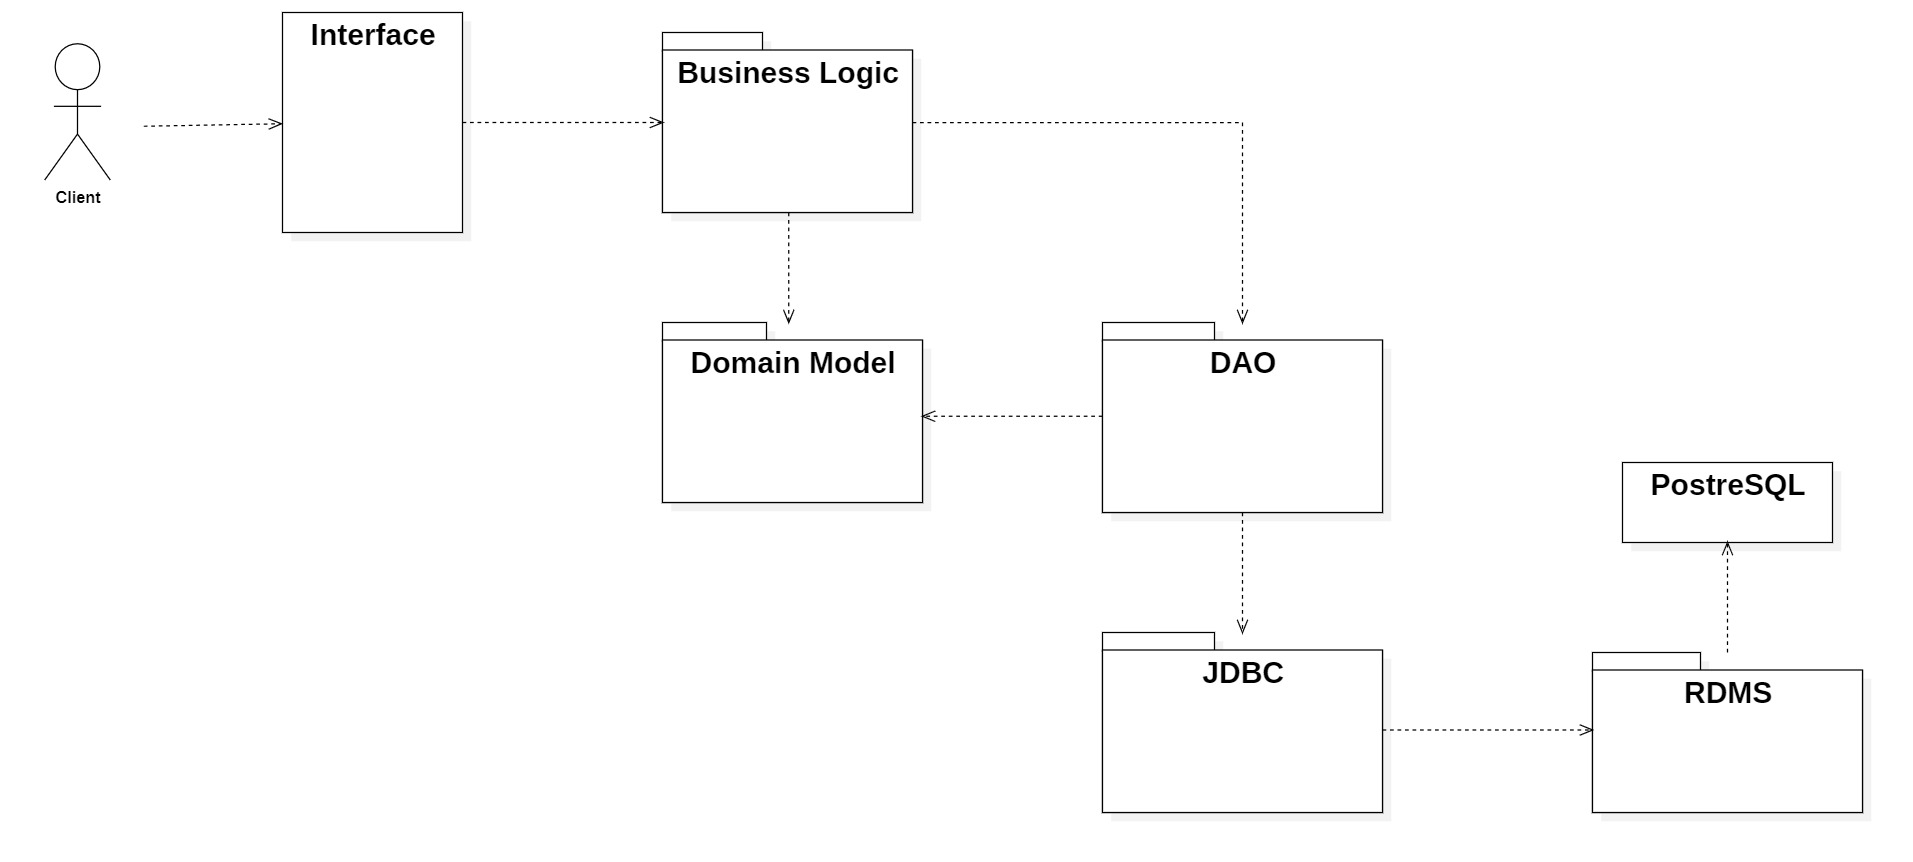
\includegraphics[scale=0.175]{Sp/Architettura}
\par\medskip
Figura 1: Diagramma dell'architettura del progetto
\par\medskip
\end{center}
L'architettura del progetto è articolata in quattro componenti:
\begin{itemize}
	\item \textbf{Business Logic}: contiene le classi che implementano la logica di business nel sistema.
	\item \textbf{Domain Model}: contiene le classi che rappresentano le entità del sistema.
	\item \textbf{ORM}: contiene le classi che permettono di gestire la comunicazione tra l'applicazione e il database andando a separare la logica per l'interazione con i dati dal resto dell'applicazione.
        \item \textbf{Interfaccia CLI}: interfaccia di linea di comando (CLI) dove l'utente può usufruire delle funzioni dell'applicazione e interagire con il sistema.
\end{itemize}
L'applicazione è stata sviluppata nel linguaggio Java e il database è stato implementato con PostrgreSQL. La connessione tra il progetto e il database è realizzata tramite JDBC. Sono state utilizzate le seguenti piattaforme e software:
\begin{itemize}
\item \textbf{IntelliJ IDEA}: IDE per lo sviluppo in Java.
\item \textbf{StarUML}: software per la creazione di diagrammi UML.
\item \textbf{Draw.io}: software per la realizzazione di altri diagrammi, tra cui il modello ER.
\item \textbf{PgAdmin}: software per la gestione del database PostgreSQL.
\item \textbf{GitHub}: piattaforma contenente il codice sorgente.
\item \textbf{Lunacy}: software per la realizzazione dei mockup.
\end{itemize}


\section{Progettazione}
\subsection{Use Case Diagram}

Sono presenti 2 tipi di utenti: lo User e l'Admin. Nel diagramma sottostante vengono rappresentati i casi d'uso per i due tipi di utenti: 
\begin{center}
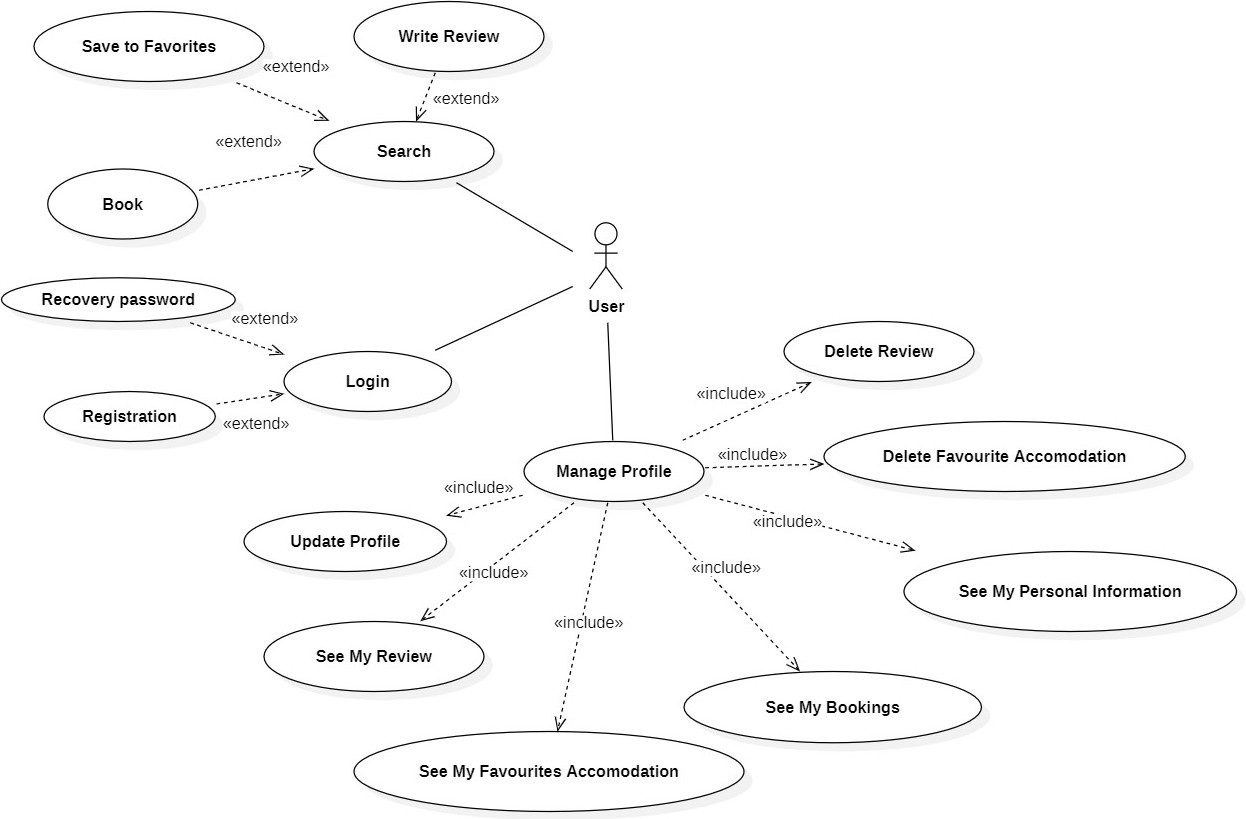
\includegraphics[scale=0.411]{usecases/ClientUseCase}
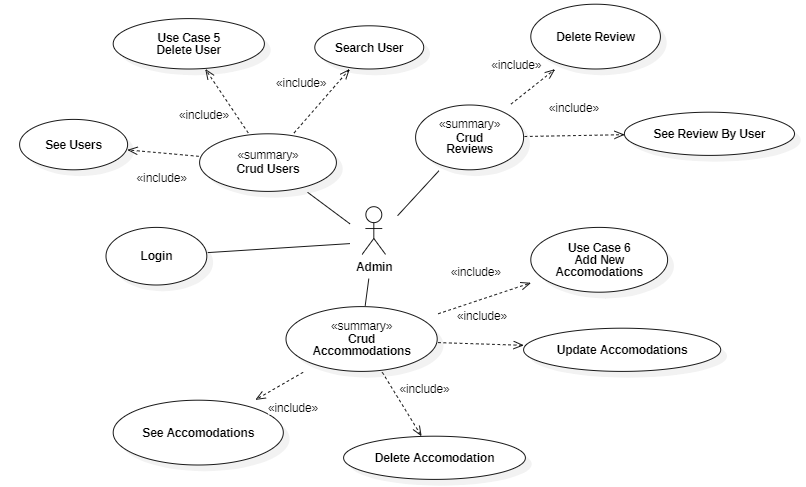
\includegraphics[scale=0.5]{usecases/AdminUseCase}\\
Figura 2: Use Case Diagram dello User e dell'Admin
\end{center}
\label{usecase}
\subsection{Use Case Template}
Sono di seguito mostrati alcuni template dei casi d'uso. In alcuni di essi sono presenti riferimenti a test e mockup presenti successivamente (sezione 2.3):

\begin{center}
\begin{table}[H]
\vspace{-0.3cm}
\centering
\scalebox{0.75}{ % Riduce tutto il blocco al 75% della dimensione originale
\begin{tabular}{|l|p{9cm}|}
\hline
\label{Usecase1}
Use Case 1 & Login (\hyperref[test1]{Tst\#1})\\ \hline
Descrizione & L'utente accede al sistema inserendo le sue credenziali. \\ \hline
Livello & Function \\ \hline
Attori & Utente, Admin \\ \hline
Flusso Base & 
\begin{enumerate}
    \item L'utente inserisce le sue credenziali (email e password) (\hyperref[mk1]{MK\#1} e \hyperref[mk3]{MK\#3}).
    \item L'utente preme il pulsante di Login.
    \item Il sistema verifica le credenziali.
    \item Il sistema autentica l'utente.
\end{enumerate} \\ \hline
Flusso Alternativo & 
\begin{enumerate}
    \item[3a.] Se le credenziali sono errate, il sistema invia un messaggio di errore.
    \item[3b.] Se si verifica un problema all'interno del database durante la ricerca dell'utente, il sistema invia un messaggio di errore.
    \item[3c] Se l'email è giusta, ma la password sbagliata, il sistema consente un recupero della password o l'immissione di un ulteriore tentativo 
    \item[4a.] Se l'accesso viene effettuato dall'utente, sarà indirizzato alla sua pagina personale.
\end{enumerate} \\ \hline
Post-condizioni & L'utente è autenticato dal sistema e ha accesso alle sue funzionalità. \\ \hline
\end{tabular}
}
\caption{Template che descrive il caso d'uso del login}
\end{table}
\begin{table}[H]
\vspace{-0.3cm}
\centering
\scalebox{0.75}{ % Riduce tutto il blocco al 75% della dimensione originale
\begin{tabular}{|l|p{9cm}|}
\hline
Use Case 2 & Search \\ \hline
Descrizione & L'utente cerca l'alloggio di suo interesse. \\ \hline
Livello & User Goal \\ \hline
Attori & User \\ \hline
Flusso Base & 
\begin{enumerate}
    \item L'utente inserisce le informazioni per effettuare la sua ricerca (\hyperref[mk6]{MK\#6}).
    \item L'utente preme il pulsante per effettuare la ricerca.
    \item Il sistema usa le informazioni per ricercare gli alloggi.
    \item Il sistema restituisce all'utente una lista di alloggi (\hyperref[mk7]{MK\#7}).
\end{enumerate} \\ \hline
Flusso Alternativo & 
\begin{enumerate}
    \item[3a.] Se l'utente non inserisce alcune informazioni necessarie alla ricerca (es: il luogo dove vuole andare, la data di check-in, la data di check-out), il sistema restituisce un messaggio di errore.
    \item[3b.] Se si verifica un problema all'interno del database durante la ricerca dell'alloggio, il sistema invia un messaggio di errore.
\end{enumerate} \\ \hline
Pre-condizioni & L'utente deve aver fatto il login. \\ \hline
Post-condizioni & L'utente riceverà una lista di alloggi da consultare. \\ \hline
\end{tabular}
}
\caption{Template che descrive il caso d'uso dello Search}
\end{table}
\begin{table}[H]
\vspace{-0.3cm}
\centering
\scalebox{0.75}{ % Riduce tutto il blocco al 75% della dimensione originale
\begin{tabular}{|l|p{9cm}|}
\hline
Use Case 3 & Book \\ \hline
Descrizione & L'utente prenota un alloggio. \\ \hline
Livello & User Goal \\ \hline
Attori & User \\ \hline
Flusso Base & 
\begin{enumerate}
    \item L'utente preme il pulsante per effettuare la prenotazione dell'alloggio (\hyperref[mk2]{MK\#2}).
    \item Il sistema riceve la richiesta di prenotazione e verifica la disponibilità dell'alloggio.
    \item Il sistema restituisce all'utente un messaggio di conferma.
\end{enumerate} \\ \hline
Flusso Alternativo & 
\begin{enumerate}
    \item[2a.] Se la disponibilità è zero, il sistema restituisce un messaggio di errore.
    \item[2b.] Se si verifica un problema durante il salvataggio della prenotazione nel database, il sistema invia un messaggio di errore.
    \item[2c.] Se l'utente non aveva inserito certi parametri per la ricerca ( data check-in check-out e numero di stanze e persone), gli verrà chiesto di inserirle per effettuare la prenotazione
\end{enumerate} \\ \hline
Pre-condizioni & L'utente deve aver fatto il login e deve aver effettuato la ricerca. \\ \hline
Post-condizioni & La prenotazione effettuata verrà aggiunta a quelle già effettuate dell'utente. \\ \hline
\end{tabular}
}
\caption{Template che descrive il caso d'uso del Book}
\end{table}
\begin{table}[H]
\vspace{-0.3cm}
\centering
\scalebox{0.75}{ % Riduce tutto il blocco al 75% della dimensione originale
\begin{tabular}{|l|p{9cm}|}
\hline
\label{Usecase4}
Use Case 4 & Registration (\hyperref[test2]{Tst\#2})\\ \hline
Descrizione & L’utente si registra all’interno del sistema.  \\ \hline
Livello & User Goal \\ \hline
Attori & User \\ \hline
Flusso Base & 
\begin{enumerate}
    \item L'utente inserisce i parametri per registrarsi (\hyperref[mk5]{MK\#5}).
    \item L'utente preme il pulsante per effettuare la registrazione.
    \item Il sistema verifica le informazioni fornite.
    \item Il sistema crea un nuovo account per l’utente.
\end{enumerate} \\ \hline
Flusso Alternativo & 
\begin{enumerate}
    \item[3a.] Se l’utente inserisce dati non validi (es: l’email già usata o vuota), il sistema invia un messaggio di errore all’utente.
    \item[3b.] Se si verifica un problema durante il salvataggio dell’utente nel database, il sistema invierà un messaggio di errore.
\end{enumerate} \\ \hline
Post-condizioni & L’utente è registrato all’interno del sistema e può accedere tramite le sue credenziali. \\ \hline
\end{tabular}
}
\caption{Template che descrive il caso d'uso del Registration}
\end{table}
\begin{table}[H]
\vspace{-0.3cm}
\centering
\scalebox{0.75}{ % Riduce tutto il blocco al 75% della dimensione originale
\begin{tabular}{|l|p{9cm}|}
\hline
Use Case 5 & Delete User \\ \hline
Descrizione & L'Admin elimina un utente dal database. \\ \hline
Livello & User Goal \\ \hline
Attori & Admin \\ \hline
Flusso Base & 
\begin{enumerate}
    \item L'admin inserisce i parametri che caratterizzano l'utente (es: Id o email).
    \item L'admin preme il pulsante per effettuare l'eliminazione dell'utente.
    \item Il sistema verifica le informazioni fornite.
    \item Il sistema elimina l'utente dal database.
\end{enumerate} \\ \hline
Flusso Alternativo & 
\begin{enumerate}
    \item[3a.] Se l'admin inserisce dati non validi, il sistema invia un messaggio di errore.
    \item[3b.] Se si verifica un problema durante l'eliminazione dell'utente dal database, il sistema invierà un messaggio di errore.
\end{enumerate} \\ \hline
Pre-condizioni & L'admin deve aver effettuato il login. \\ \hline
Post-condizioni & L'utente è stato eliminato con successo e non può più accedere all'applicazione a meno che non venga effettuata una nuova registrazione. \\ \hline
\end{tabular}
}
\caption{Template che descrive il caso d'uso del Delete User}
\end{table}
\begin{table}[H]
\centering
\scalebox{0.75}{ % Riduce tutto il blocco al 75% della dimensione originale
\begin{tabular}{|l|p{9cm}|}
\hline
Use Case 6 & Add Accommodation \\ \hline
Descrizione & L'admin aggiunge un nuovo alloggio al database. \\ \hline
Livello & User Goal \\ \hline
Attori & Admin \\ \hline
Flusso Base & 
\begin{enumerate}
    \item L'admin inserisce i parametri che caratterizzano l'alloggio.
    \item L'admin preme il pulsante per effettuare l'aggiunta dell'alloggio.
    \item Il sistema verifica le informazioni fornite.
    \item Il sistema registra l'alloggio appena inserito.
\end{enumerate} \\ \hline
Flusso Alternativo & 
\begin{enumerate}
    \item[3b.] Se si verifica un problema durante la registrazione dell'alloggio nel database, il sistema invia un messaggio di errore.
\end{enumerate} \\ \hline
Pre-condizioni & L'admin deve aver fatto il login. \\ \hline
Post-condizioni & L'alloggio è stato registrato con successo e sarà disponibile per le successive ricerche degli utenti. \\ \hline
\end{tabular}
}
\caption{Template che descrive il caso d'uso dell'Add Accomodation}
\end{table}
\end{center}


\subsection{Mockups}
Sono riportati alcuni mockup, realizzati con \textbf{Lunacy}, relativi ad una possibile interfaccia grafica per l'applicazione:
\begin{center}
\phantomsection
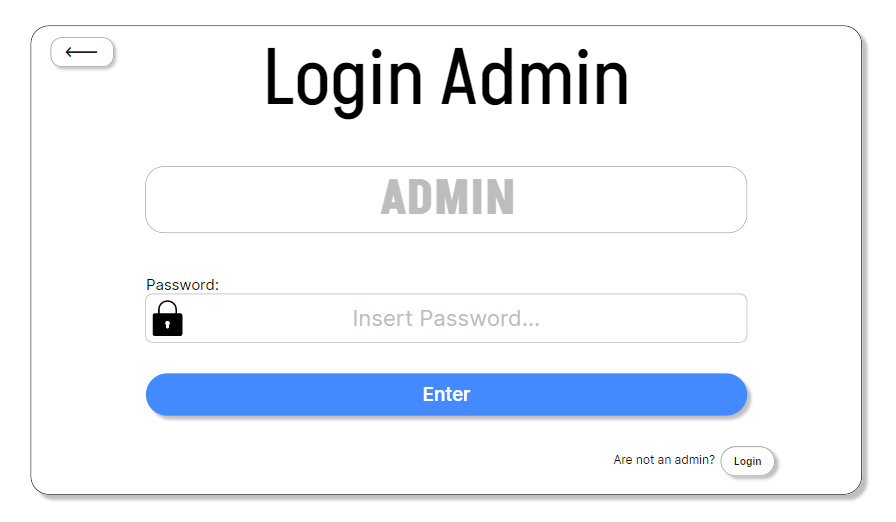
\includegraphics[scale=0.6]{Mockup/MockupAdminLogin}
\label{mk1}
\par\medskip
Figura 3: Mockup per il login effettuato da un admin - MK\#1 
\par\medskip
\par\medskip
\phantomsection
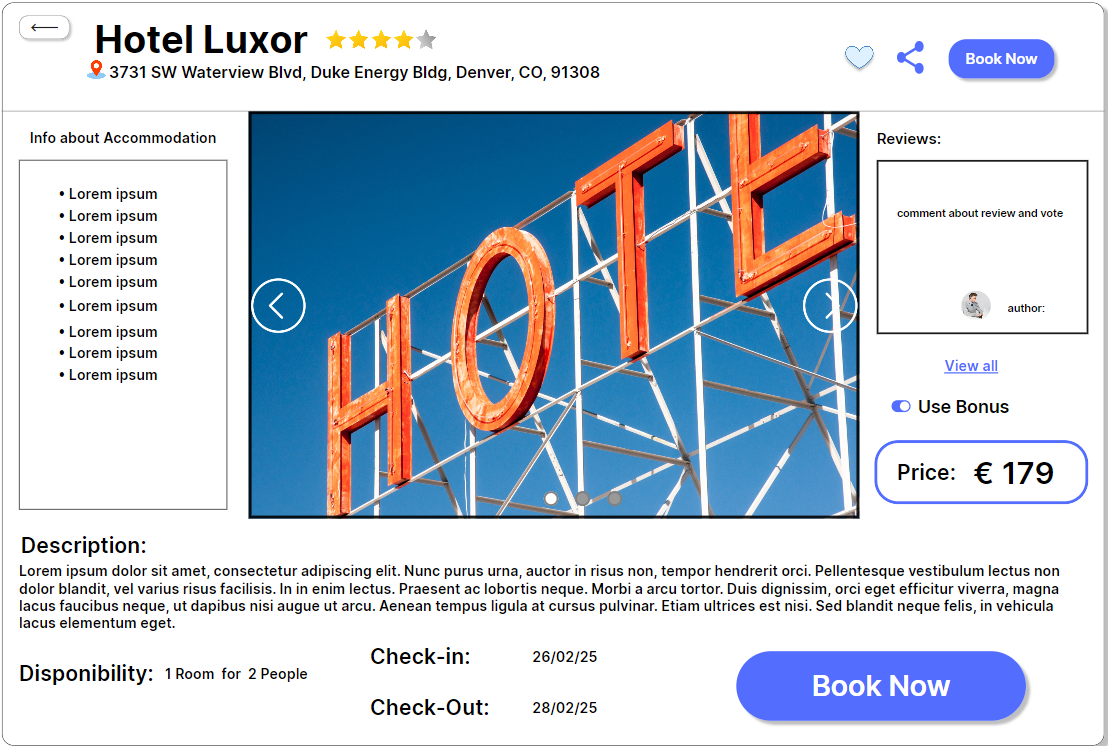
\includegraphics[scale=0.5]{Mockup/mockupBooking}
\label{mk2}
\par\medskip
\par\medskip
Figura 4: Mockup per mostrare in dettaglio un alloggio con la possibilità di prenotarlo - MK\#2
\par\medskip
\phantomsection
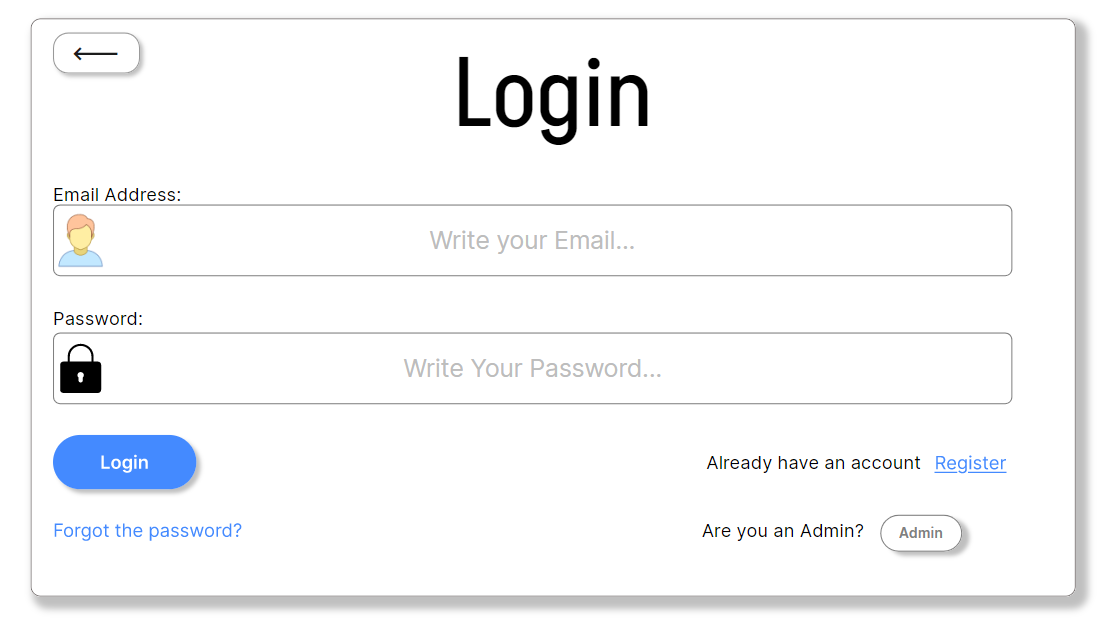
\includegraphics[scale=0.5]{Mockup/MockupLogin}
\label{mk3}
\par\medskip
Figura 5: Mockup per il login effettuato da un utente - MK\#3
\par\medskip
\phantomsection
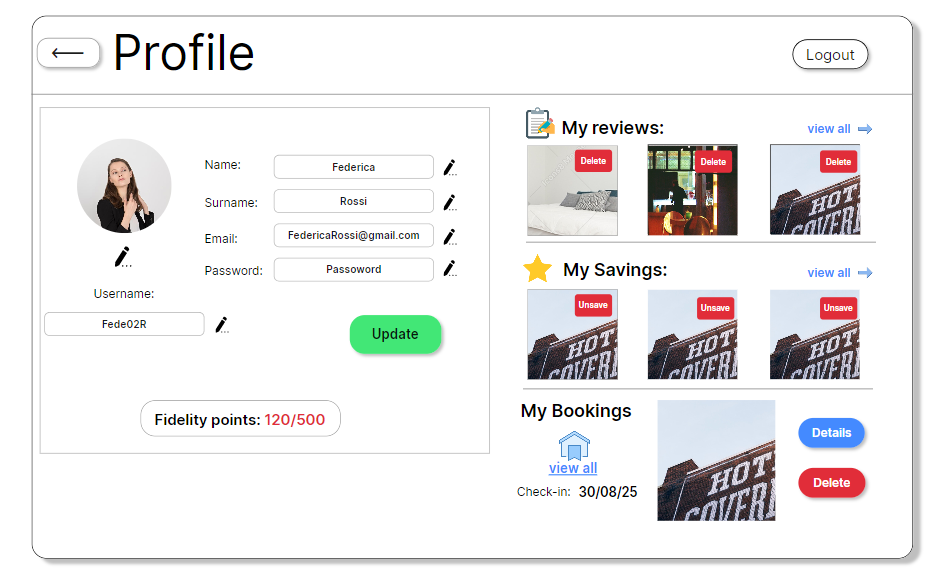
\includegraphics[scale=0.6]{Mockup/MockupProfile}
\label{mk4}
\par\medskip
Figura 6: Mockup per mostrare il profilo di un utente - MK\#4
\par\medskip
\phantomsection
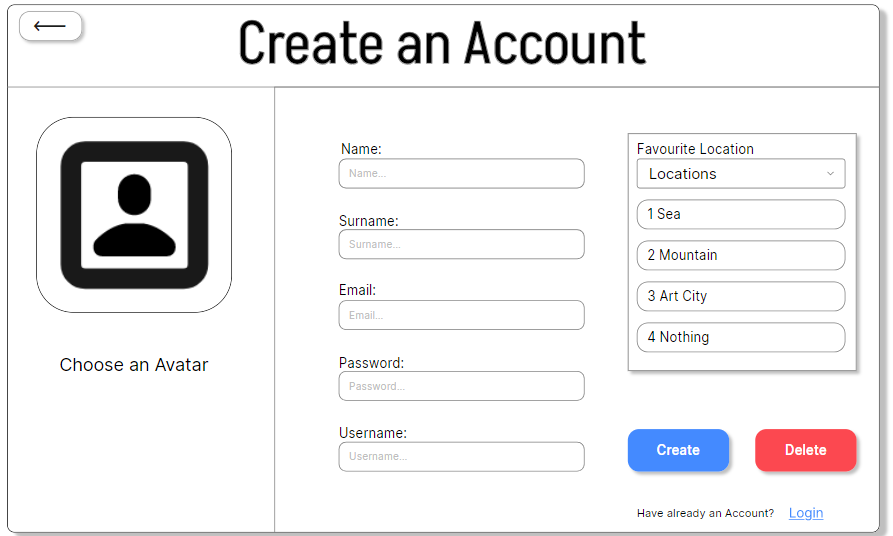
\includegraphics[scale=0.6]{Mockup/MockupRegister}
\label{mk5}
\par\medskip
\par\medskip
Figura 7: Mockup per creare un account - MK\#5
\par\medskip
\par\medskip
\phantomsection
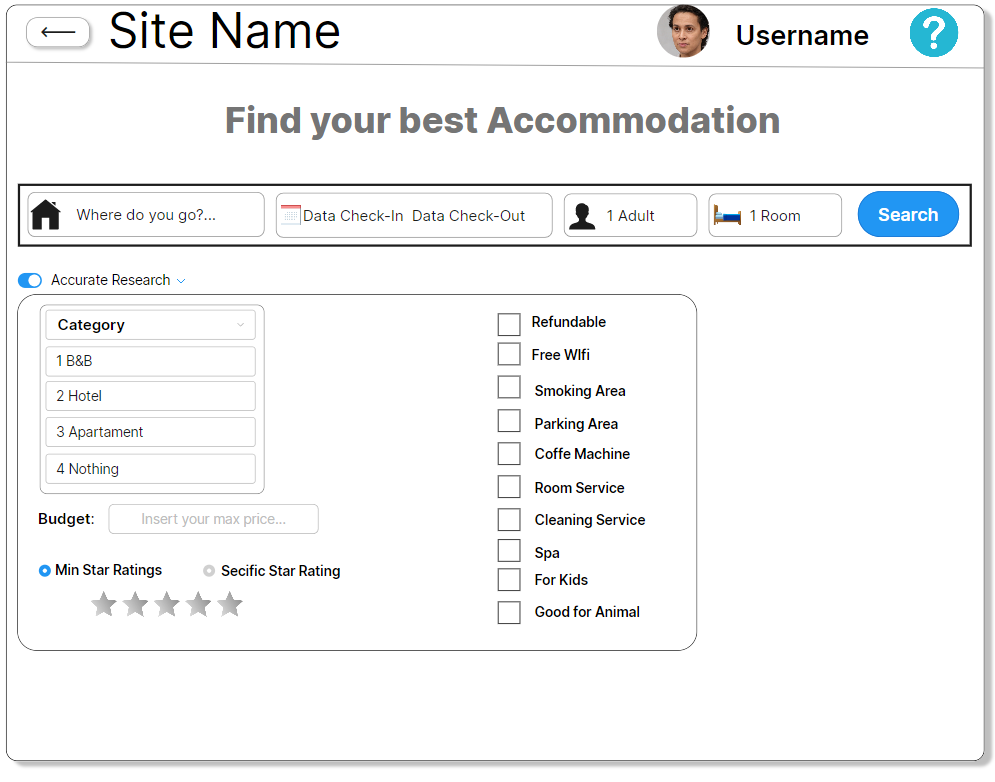
\includegraphics[scale=0.55]{Mockup/MockupResearch}
\label{mk6}
\par\medskip
Figura 8: Mockup per effettuare la ricerca attraverso i filtri - MK\#6
\par\medskip
\phantomsection
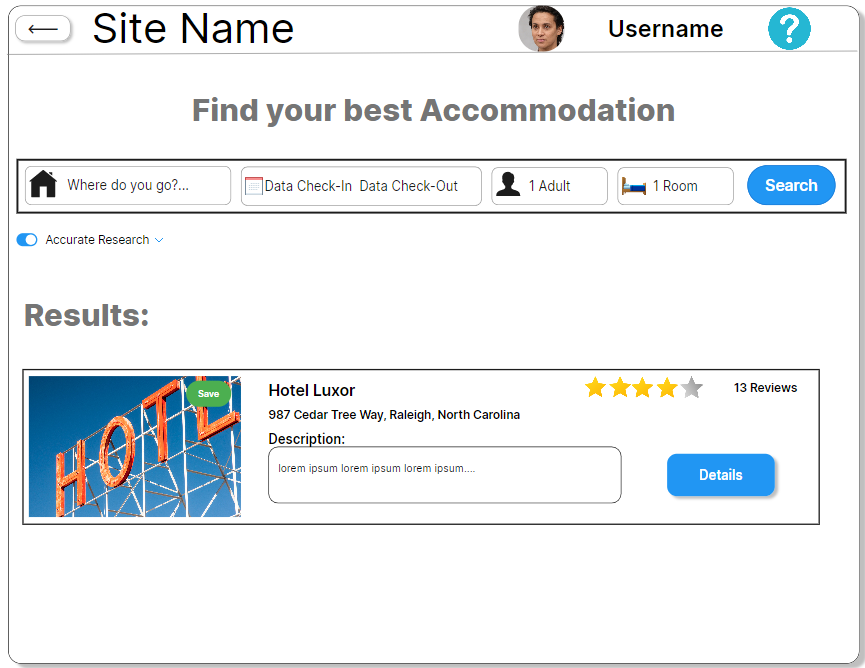
\includegraphics[scale=0.6]{Mockup/MockupResult}
\label{mk7}
\par\medskip
Figura 9: Mockup che mostra i risualtati di una ricerca - MK\#7
\par\medskip
\end{center}

\subsection{Class Diagram}
L'architettura è divisa in 3 package:
\begin{itemize}
\label{domainmodel}
\item \textbf{Domain Model}: consiste nell’insieme di classi che rappresentano i concetti con cui interagisce l’applicazione: \textbf{RegisterUser}, \textbf{Review}, \textbf{Booking}, \textbf{Accommodation}, \textbf{SearchParameters} e \textbf{SearchParametersBuilder}.
\par\medskip
\hspace*{-0.5cm}
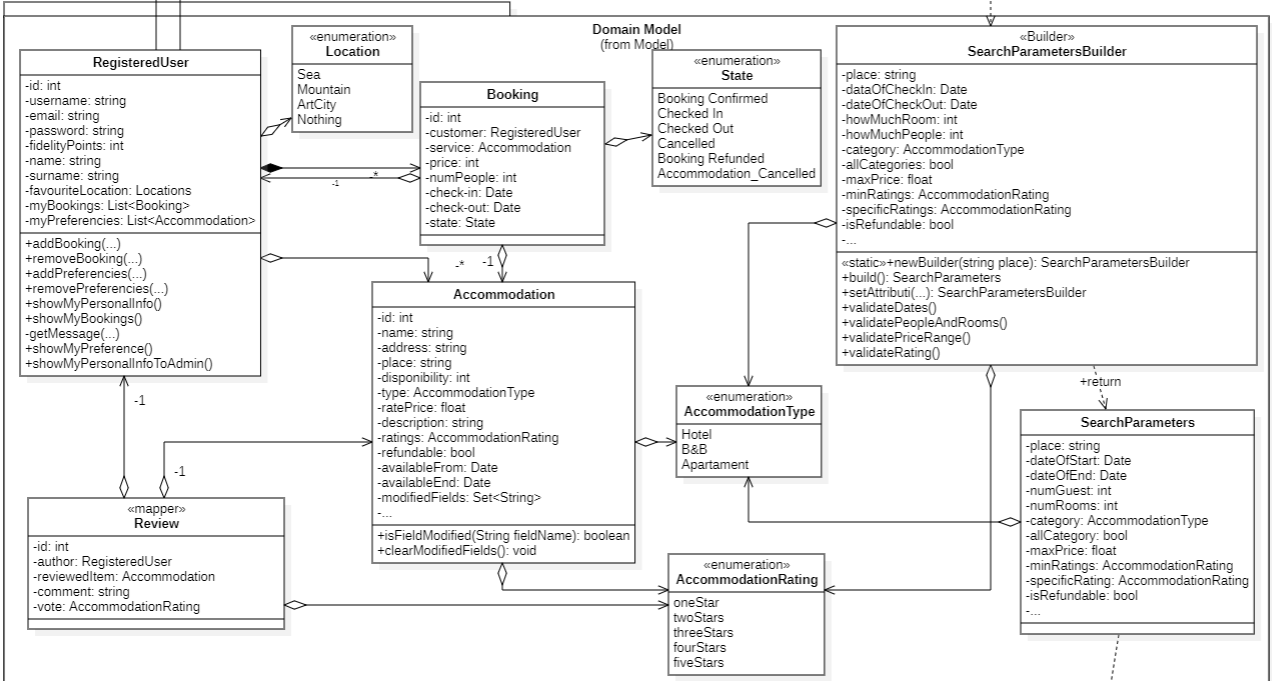
\includegraphics[scale=0.58]{uml/DomainModel}
\par\medskip
\begin{center}
Figura 11: Class Diagram - Domain Model 
\end{center}
\par\medskip
\vspace{-0.3cm}
\item \textbf{ORM}: è il package che si occupa di gestire la connessione con il database: \textbf{UserDAO}, \textbf{BookingDAO}, \textbf{PreferenceDAO}, \textbf{ReviewDAO}, \textbf{AccommodationDAO}, \textbf{DatabaseConnection}.
\par\medskip
\hspace*{-0.5cm}
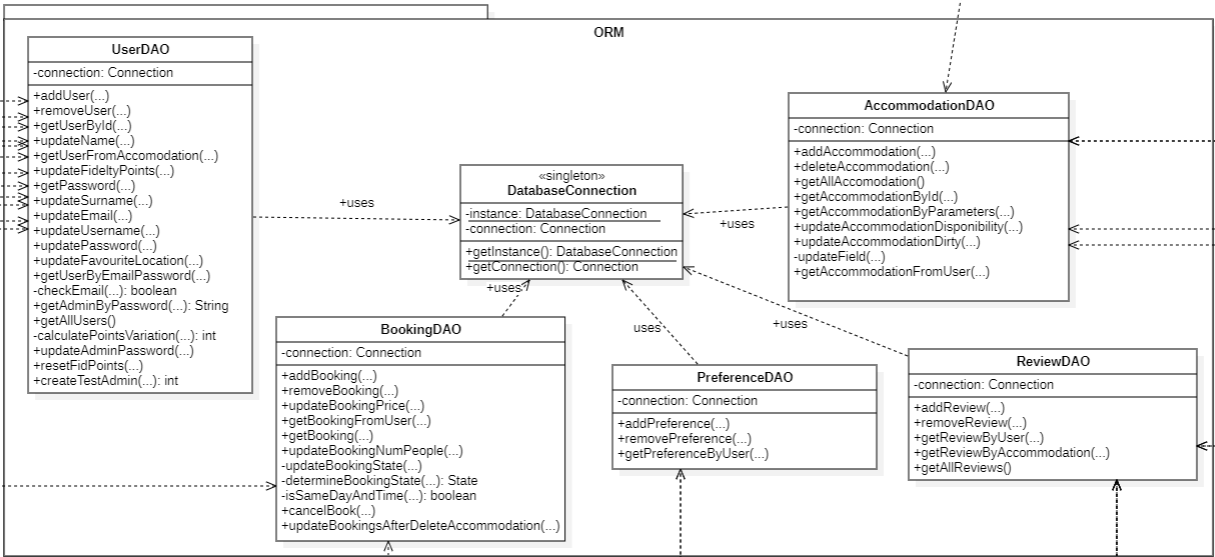
\includegraphics[scale=0.58]{uml/DAO}
\par\medskip
\begin{center}
Figura 12: Class Diagram - ORM
\end{center}
\par\medskip
\item \textbf{Business Logic}: è il package che contiene i controller, che sono 4: quello che gestisce l'accesso, la registrazione e un eventuale recupero password (\textbf{UserController}), quello che gestisce il profilo dell'utente e una sua eventuale rimozione(\textbf{ProfileUserController}), quello che gestisce la logica dell'applicazione (ricerca, prenotazione, recensione) (\textbf{ResearchController}) e quello che gestisce le azioni che può effettuare l'Admin (\textbf{AdminController}).  
\par\medskip
\hspace*{-0.75cm}
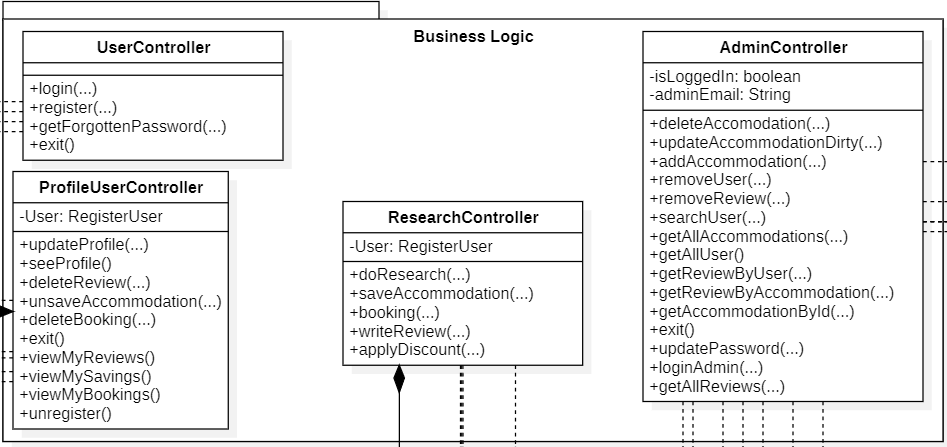
\includegraphics[scale=0.6]{uml/BusinessLogic}
\begin{center}
Figura 10: Class Diagram - Business Logic 
\end{center}

\end{itemize}
\subsection{Dettagli di Progetto}
Nell'architettura sono stati usati diversi design pattern:
\subsubsection{Singleton}

Il Singleton è stato utilizzato per garantire che la connessione al database venisse effettuata una singola volta e per evitare conflitti tra connessioni.
\par\medskip
\vspace{-0.3cm}
\begin{center}
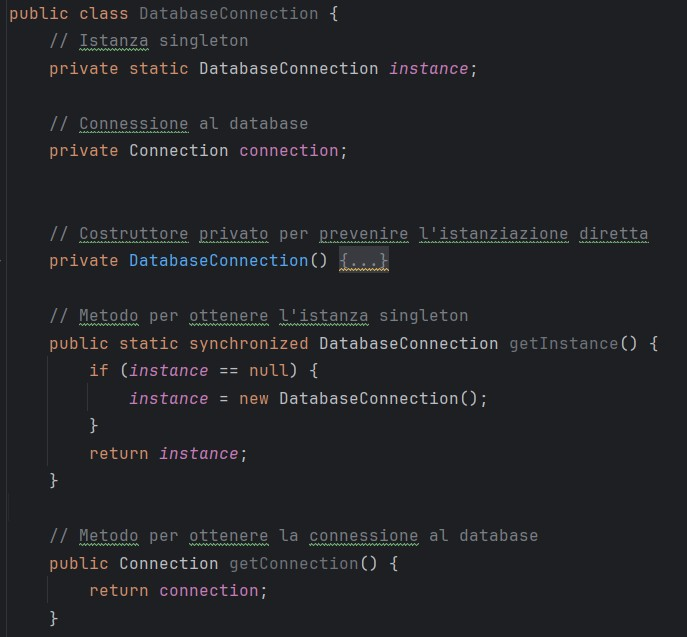
\includegraphics[scale=0.65]{Snippets/Singleton}
\par\medskip
Snippet 1: Implementazione Singleton
\par\medskip
\end{center}

\subsubsection{Mapper}

Lo scopo del Mapper è quello di creare la relazione tra utenti, recensioni e alloggi.

\begin{center}
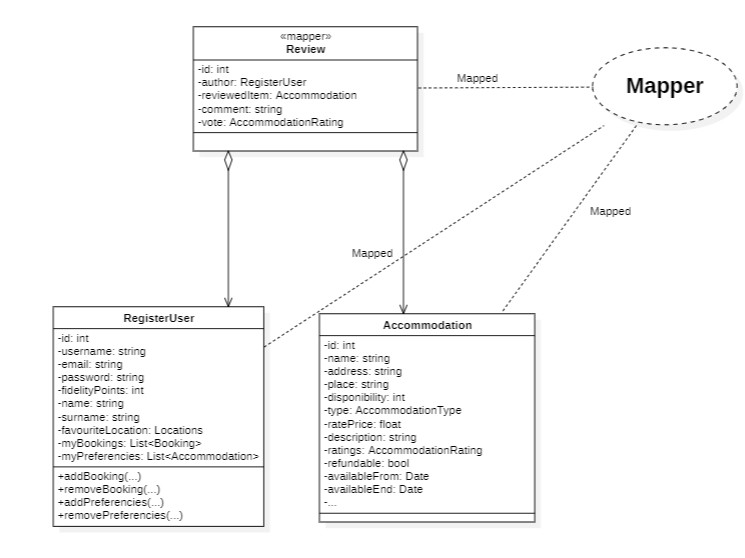
\includegraphics[scale=0.75]{Snippets/Mapper}
\par\medskip
Snippet 2: UML del Mapper
\par\medskip
\end{center}

\subsubsection{Builder Telescoping Constructor}

Il Builder Telescoping Constructor viene usato per creare la classe parametri di ricerca che presenta tanti attributi, spesso opzionali, e ne consente una gestione più efficiente. L'unico scopo della classe è quello creare un oggetto di tipo ParametriRicerca e ci riesce grazie ai metodi di setting, che ritornando la classe stessa, consentono di avere una chiara creazione dell'oggetto, attraverso un metodo statico e evitando l'overloading dei costruttori tradizionali (\textbf{build}). La classe per definizione presenta tutti gli attributi della classe \textbf{SearchParameters} quindi possiede 19 attributi e ognuno di essi ha implementato un setter. Inoltre, per funzionare, creare una classe \textbf{SearchParametersBuilder} bisogna fornigli un valore di tipo String che nel nostro progetto rappresenta il luogo della ricerca (\textbf{newBuilder(String place)}). Per evitare che l'utente creasse dei parametri di ricerca invalidi abbiamo inserito nella fase di build dei metodi di validazione che lanciano delle eccezioni quando l'utente sbaglia a inserire un valore. Un esempio può essere la validazione delle date che controlla che l'utente non abbia inserito nella ricerca date passate.
Per implemenentare questa classe sono state richieste circa 203 linee di codice. Qui sottostante ne riporteremo alcune più significative
\newpage
\UseRawInputEncoding
\begin{lstlisting}
public final class SearchParametersBuilder {
    private final String place;
    private LocalDateTime dateOfCheckIn;
    private LocalDateTime dateOfCheckOut;
    private Integer howMuchRooms=0;
    private Integer howMuchPeople=0;
    private AccommodationType category;
    private boolean allCategories;
    private Float maxPrice=0.0f;
    private AccommodationRating minAccommodationRating;
    private AccommodationRating specificAccommodationRating;
    private boolean isRefundable;
    private boolean haveFreeWifi;
    private boolean canISmoke;
    private boolean haveParking;
    private boolean haveCoffeeMachine;
    private boolean haveRoomService;
    private boolean haveCleaningService;
    private boolean haveSpa;
    private boolean goodForKids;
    private boolean canHaveAnimal;

    public SearchParametersBuilder setDateOfCheckIn(LocalDateTime dateOfCheckIn) {
        this.dateOfCheckIn = dateOfCheckIn;
        return this;
    }
    // ...
    
    private SearchParametersBuilder(String place) {
        this.place = place;
    }

    public static SearchParametersBuilder newBuilder(String place){
        if(place.trim().isEmpty()){
            throw new IllegalArgumentException("Place cannot be empty");
        }
        return new SearchParametersBuilder(place);
    }

    public SearchParameters build() {

        // Validazione delle date
        validateDates();

        // Validazione degli altri parametri
        validatePeopleAndRooms();
        validatePriceRange();
        validateRating();

        return new SearchParameters(place,  dateOfCheckIn,  dateOfCheckOut,  howMuchRooms,  howMuchPeople, category,  allCategories,  maxPrice, minAccommodationRating, specificAccommodationRating,  isRefundable,  haveFreeWifi,  canISmoke,  haveParking,  haveCoffeeMachine,  haveRoomService,  haveCleaningService,  haveSpa,  goodForKids,  canHaveAnimal);
    }

    private void validateDates() {
        LocalDateTime now = LocalDateTime.now();

        if (dateOfCheckIn != null && dateOfCheckOut != null) {
            // Verifica che le date non siano nel passato
            if (dateOfCheckIn.isBefore(now)) {
                throw new IllegalArgumentException("Check-in date cannot be in the past.");
            }

            if (dateOfCheckOut.isBefore(now)) {
                throw new IllegalArgumentException("Check-out date cannot be in the past.");
            }

            // Verifica che la data di check-out sia dopo il check-in
            if (!dateOfCheckOut.isAfter(dateOfCheckIn)) {
                throw new IllegalArgumentException("Check-out date must be after check-in date.");
            }

        } else if (dateOfCheckIn != null || dateOfCheckOut != null) {
            // Se solo una delle due date è specificata
            throw new IllegalArgumentException("Both check-in and check-out dates must be provided or both must be null.");
        }
    }
    //...
\end{lstlisting}
\par\medskip
\label{daosec}
\subsubsection{DAO}

Il DAO (Data Access Object) \`e un design pattern che si occupa di separare le classi che si interfacciano al database dall'applicazione. Questo viene fatto
per poter meglio implementare il principio di singola responsabilit\`a e aumenta
la mantenibilità del codice. Viene implementato nel package ORM.

\subsection{ER Diagram e Relational Model}

Per il database e la sua gestione, \`e stato realizzato un ER Diagram (Figura 13), e il Relational Model derivato (Figura 14), entrambi realizzati con \textbf{Draw.io}. Ci sono state delle scelte progettuali precise, in particolare quella riguardante l'entit\`a \textbf{Alloggio}, dove per differenziare i tipi di alloggio è stato usato un attributo al posto di una generalizzazione, dovuto al fatto che nel progetto si faranno uso di informazioni che sono a comune tra i vari alloggi, favorendo accessi più veloci ma a discapito di un notevole spreco di memoria e la presenza di valori nulli.\\
Alla fine sono state definite le seguenti tabelle:
\begin{itemize}
\item \textbf{User}: rappresenta l'entità \textbf{User}.
\item \textbf{Booking}: rappresenta l'entità \textbf{Booking}.
\item \textbf{Acccommodation}: rappresenta l'entità \textbf{Accommodation}.
\item \textbf{Review}: rappresenta la relazione \textbf{Review} che avviene tra l'entità \textbf{User} e l'entità \textbf{Accommodation}.
\item \textbf{Favourites}: rappresenta la relazione \textbf{Like} che avviene tra l'entità \textbf{User} e l'entità \textbf{Accommodation}.
\end{itemize}
\begin{center}
\par\medskip
\hspace*{-2cm}
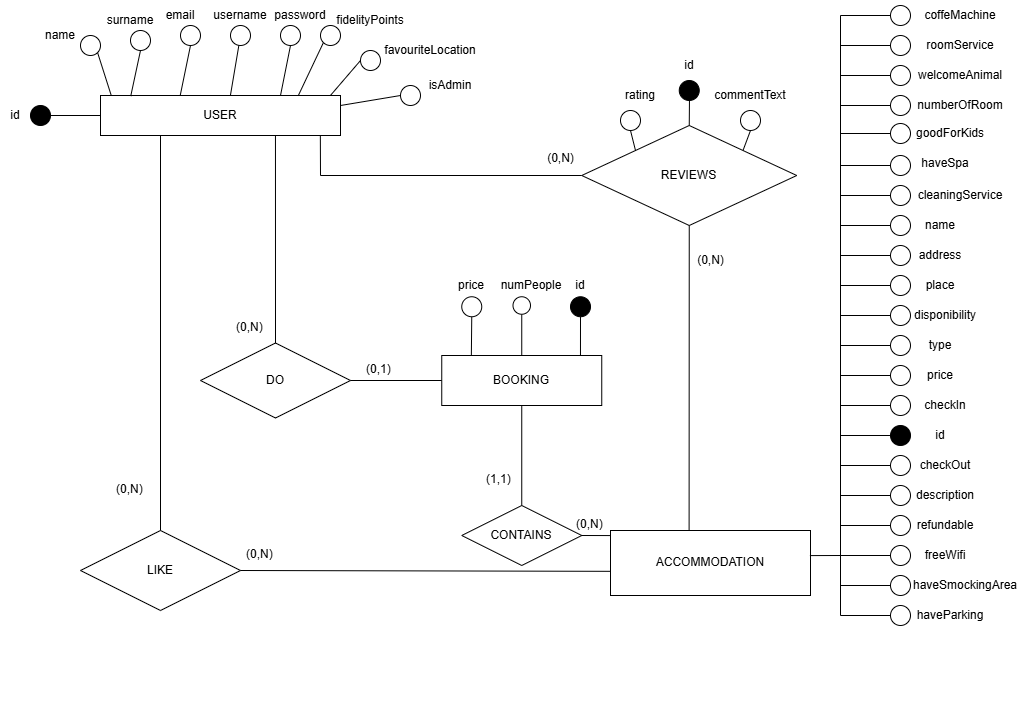
\includegraphics[scale=0.41]{ERimages/FinalER}
\par\medskip
Figura 13: ER Diagram
\par\medskip
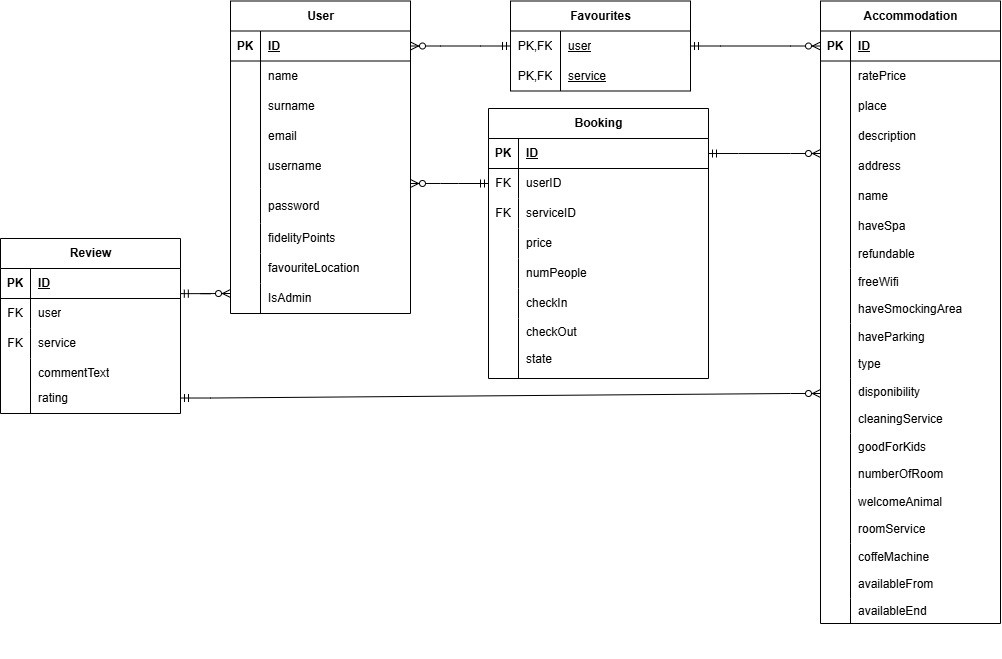
\includegraphics[scale=0.5]{ERimages/schemaLogicoDBTabelle}
\par\medskip
Figura 14: Tables of the database
\par\medskip
\end{center}

\subsubsection{Dettagli implementativi del database}

Per gestire l'update del rating dell'alloggio all'interno del database è stata optata come soluzione l'utilizzo dei trigger. Il rating dell'alloggio viene aggiornato ogni volta che viene aggiunta o eliminata una sua recensione aggiornandone il valore con la media dei rating delle sue recensioni.

\begin{center}
\par\medskip
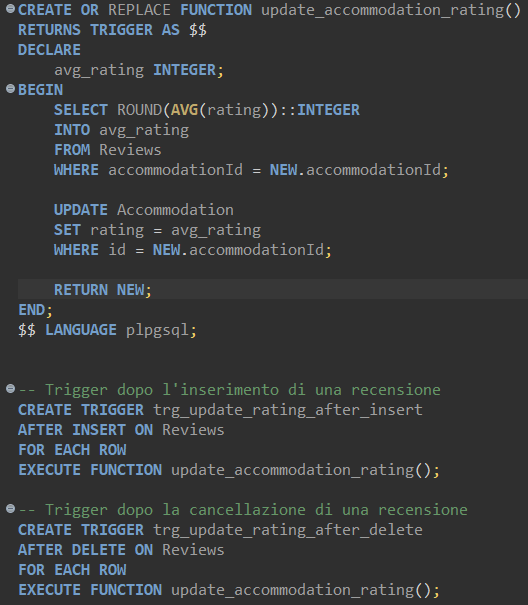
\includegraphics[scale=0.65]{trigger/trigger}
\par\medskip
Figura 15: trigger implementati per l'aggiornamento del rating per gli alloggi.
\par\medskip
\end{center}

\section{Implementazione}
\subsection{Business Logic}

\`E il package che contiene i controller e che espone all'esterno le funzionalità dell'applicazione. \`E responsabilità dei controller gestire le dipendenze tra gli oggetti creati dai DAO. I controller accedono alle funzionalità del DAO grazie ai loro metodi dove vengono instanziati le classi DAO necessarie. La loro relazione si può rappresentare come la dipendenza d'uso.
Qui sotto mostriamo un esempio di come comunica un controller con il DAO:
\clearpage
\begin{lstlisting}
public class ResearchController {
    private RegisteredUser user;
    //...
    //metodo per effettuare la ricerca
    public ArrayList<Accommodation> doResearch(SearchParameters SP) {
        //istanziamento del DAO necessario
        AccommodationDAO accommodationDAO = new AccommodationDAO();  
        return accommodationDAO.getAccommodationByParameter(SP);
    }
    //...
\end{lstlisting}
\par\medskip
\begin{center}
Frammento di codice del ResearchController implementazione della ricerca degli alloggi
\par\medskip
\end{center}
\subsubsection{UserController}

\`E la classe che si occupa di implementare le funzionalità di un utente generico per l'accesso all'applicazione. Infatti presenta i metodi di login, di registrazione e un eventuale recupera password.

\subsubsection{ProfileController}

\`E la classe che si occupa di gestire le informazioni del profilo utente e dei servizi di cui ha usufruito (\textbf{deleteReview()}, \textbf{deleteBooking()}, \textbf{unsaveAccommodation()}, \textbf{viewMySavings()}, \textbf{viewMyReviews()}, \textbf{viewMyBookings()}).

\subsubsection{ResearchController}

\`E la classe che si occupa di fornire i metodi che implementano la logica dell'applicazione. Infatti, permette la ricerca in base a dei parametri (\textbf{doResearch()}) e sugli alloggi ricercati permette, a un utente registrato, di effettuare una prenotazione (\textbf{booking()}), salvarlo tra i preferiti (\textbf{saveAccomodation()}) e scrivere una recensione su quell'alloggio (\textbf{writeReview()}). Per funzionare, oltre ai collegamenti ai relativi DAO, questa classe usa il \textbf{SearchParametersBuilder} che si trova nel \textbf{Domain Model}.

\subsubsection{AdminController}

\`E la classe che si occupa di implementare le operazioni dell'admin, il quale può  leggere, modificare, cancellare e aggiungere alloggi, mentre può solo leggere e cancellare utenti e recensioni.
 
\subsection{Domain Model}

\`E il package che rappresenta il modello dei dati e implementa le classi che raffigurano le entità del sistema.

\subsubsection{RegisterUser}

Contiene le informazioni relative all'utente registrato. Gli attributi della classe sono: id (utilizzato come identificativo), username, email (unica all'interno dell'applicazione), password, nome, cognome, punti fedeltà (che si aggiornano ad ogni acquisto e raggiunta una certa soglia, permette di avere degli sconti), località preferita che indica un genere di esperienza che preferisce, la lista delle prenotazioni effettuate e la lista dei suoi alloggi preferiti. 

\subsubsection{Booking}

\`E la classe che rappresenta l'entità prenotazione, con tutte le informazioni relative ad essa. Possiede un id identificativo, l'acquirente, il servizio, per quante persone è la prenotazione, il prezzo, il check-in, il check-out e lo stato della prenotazione.

\subsubsection{Accommodation}

\`E la classe che rappresenta l'entità alloggio e tiene conto dei suoi attributi. Molti dei suoi attributi non sono obbligatori, ma dipendono dai servizi che offre l'alloggio. Ha un id (univoco), un nome, un indirizzo, un luogo, quante persone possono alloggiarci, tipo di alloggio (B\&B, appartamento e hotel), il prezzo, il periodo di disponibilità, la descrizione di cosa offre, un insieme di stringhe che permette di sapere cosa è stato modificato e diversi parametri aggiuntivi che non sono obbligatori (visualizzabili nelle \hyperref[domainmodel]{figure} precedenti) .

\subsubsection{Review}

\`E la classe che rappresenta l'entità recensione. I campi sono id, autore, alloggio recensito, commento e il voto. Consente di stabilire una correlazione tra l'utente e l'alloggio in maniera discreta, senza che tale connessione sia direttamente percepita dagli interessati.

\subsubsection{SearchParametersBuilder e SearchParameters}

Queste classi implementano il design pattern Builder Telescopic Constructor per la creazione dei parametri di ricerca. Il \textbf{SearchParametersBuilder} consente una creazione più facile da gestire e da estendere dei parametri di ricerca. Infatti il suo unico scopo è di creare la classe \textbf{SearchParameters}. Quest'ultima classe possiede solo gli attributi che poi serviranno alla ricerca all'interno del database. Gli attributi sono per la maggior parte uguali alla classe \textbf{Accommodation}.

\subsection{ORM}

\`E il package che implementa il design pattern DAO descritto nella sezione \hyperref[daosec]{2.5.4}. Le classi in questo package permettono alle classi presenti nella \textbf{Business Logic} di accedere ai vari dati di loro interesse nel database. Ogni classe possiede un attributo di tipo Connection, tipo del \textbf{JDBC} che rappresenta la connessione al database ottenuta dalla classe \textbf{DatabaseConnection}.
\newline
\begin{lstlisting}
public class AccommodationDAO {
  private Connection connection;
  public AccommodationDAO() {
     try {
         this.connection = DatabaseConnection.getInstance().getConnection();
        } catch (Exception e) {
         System.err.println(e.getMessage());
        }
    }
    //...
\end{lstlisting}
\begin{center}
\par
Esempio di come una classe DAO ottiene la connessione al db
\par\medskip
\end{center}
Per la complessità dell'applicazione stessa le classi DAO devono comunicare tra loro e lo fanno passando dai controller della \textbf{Business Logic}. Esistono alcuni metodi che per comunicare non passano dal controller, ma vengono richiamati direttamente dalla classe DAO stessa per una questione di comodità. Un esempio è il metodo \textbf{getUserByEmailPassword(...)} del \textbf{UserDAO}.
\newline
Qui sotto mostriamo un esempio di comunicazione passando dai controller:
\begin{lstlisting}
// cancella una prenotazione ma non la rimuove e attiva tutte le funzioni del caso
    public void cancelABooking(Booking booking) {
        BookingDAO bookingDAO=new BookingDAO();
        bookingDAO.cancelBook(booking);
        AccommodationDAO accommodationDAO=new AccommodationDAO();
        UserDAO userDAO=new UserDAO();
        userDAO.updateFidPoints(user, -booking.getPrice());
        accommodationDAO.updateAccommodationDisponibility(
          booking.getAccommodation().getId(),
          booking.getAccommodation().getDisponibility()+1
            );
    }
\end{lstlisting}
\begin{center}
\par
Codice di cancellazione di una prenotazione nel ProfileUserController in cui si usa BookingDAO, UserDAO, AccommodationDAO
\par\medskip
\end{center}
\subsubsection{DatabaseConnection}

\`E la classe che si occupa di gestire la connessione al database per le altre classi DAO tramite il metodo \textbf{getConnection()}. Classe implementata usando il design pattern \textit{Singleton} per evitare conflitti tra connessioni.

\subsubsection{UserDAO}

\`E la classe che si occupa della gestione dei dati degli utenti. Questa classe contiene molti metodi, offrendo la possibilità di aggiungere nuovi utenti e di rimuovere quelli già presenti nel database (rispettivamente \textbf{addUser()} e \textbf{removeUser()}), la possibilità di recuperare un utente tramite l'id identificativo (\textbf{getUserById()}). Infine la classe presenta i metodi che permettono di aggiornare i dati personali di un utente e di eliminarlo.
\newline
Esempio

\subsubsection{BookingDAO}

\`E la classe che si occupa della gestione dei dati che riguardano le prenotazioni effettuate dagli utenti. La classe mette a disposizione metodi che permetto di aggiungere o rimuovere delle prenotazioni (rispettivamente \textbf{addBooking()} e \textbf{removeBooking()}), di visualizzare le prenotazioni fatte da uno specifico utente (\textbf{getBookingFromUser()}) e di modificare lo stato della prenotazione.
\par\medskip
\begin{lstlisting}
public Booking addBooking(RegisteredUser user, Accommodation accommodation, LocalDateTime datein, LocalDateTime dateout, int nPeople, int price) {
    if(accommodation.getDisponibility()==0){
        throw new RuntimeException("This accommodation is not disponible");
    }
    PreparedStatement preparedStatement=null;
    try {
        String query="insert into booking (userid,accommodationid,checkin,checkout,price,
        numpeople, state) values(?,?,?,?,?,?,?) RETURNING id";
        
        preparedStatement=connection.prepareStatement(query);
        preparedStatement.setInt(1, user.getId());
        preparedStatement.setInt(2, accommodation.getId());
        preparedStatement.setTimestamp(3, java.sql.Timestamp.valueOf(datein));
        preparedStatement.setTimestamp(4, java.sql.Timestamp.valueOf(dateout));
        preparedStatement.setInt(5, price);
        preparedStatement.setInt(6, nPeople);
        preparedStatement.setString(7,
                State.Booking_Confirmed.name());
        ResultSet rs = preparedStatement.executeQuery();
        if(rs.next()) {
            return new Booking( rs.getInt(1), user, accommodation, price, nPeople, datein, 
            dateout, State.Booking_Confirmed);
            }
    } catch (SQLException e) {
        DBUtils.printSQLException(e);
    }finally{
        DBUtils.closeQuietly(preparedStatement);
    }
    return null;
}
\end{lstlisting}
\begin{center}
    \par
Query che inserisce un record di booking nel database e che ne restituisce un'istanza nel codice
    \par\medskip
\end{center}
\subsubsection{PreferenceDAO}

\`E la classe che si occupa della gestione dei dati che riguardano le liste di alloggi preferiti dagli utenti, i quali posso essere visionati senza dover fare una nuova ricerca. Questa classe contiene i metodi che permettono di aggiungere un nuovo alloggio tra i preferiti (\textbf{addPreference()}), di rimuovere un alloggio tra i preferiti (\textbf{removePreference()}) e di visualizzare gli alloggi preferiti di uno specifico utente (\textbf{getPreferenceByUser()}). 

\subsubsection{ReviewDAO}

\`E la classe che si occupa della gestione delle recensioni scritte sugli alloggi da parte degli utenti. La classe contiene i metodi che permettono di aggiungere nuove recensioni (\textbf{addReview()}), di rimuovere le recensioni dall'applicazione (\textbf{removeReview()}), e di visualizzare le recensioni scritte da uno specifico utente (\textbf{getReviewByUser()}) o visualizzare le tutte le recensioni scritte su uno specifico alloggio (\textbf{getReviewByAccommodation()}). 

\subsubsection{AccommodationDAO}

\`E la classe che si occupa della gestione dei dati degli alloggi. Questa classe presenta molti metodi, permettendo di aggiungere nuovi alloggi \newline(\textbf{addAccommodation()}), di rimuovere gli alloggi gia' presenti \newline(\textbf{deleteAccommodation()}), di visualizzare tutti gli alloggi
\newline(\textbf{getAllAccommodation()}), di visualizzare uno nello specifico tramite il suo identificativo (\textbf{getAccommodationById()}, questo metodo è molto utile per la gestione degli alloggi da parte dell'admin) e di visualizzare gli alloggi che vengono ricercati tramite l'uso dei filtri (\textbf{getAccommodationByParameters()}). Infine sono presenti i 2 metodi che permettono di aggiornare i dati di un alloggio attraverso l'uso di un insieme di stringhe per evitare accessi inutili al database (\textbf{updateAccommodationDirty()}, \textbf{updateField()}).
Qui di seguito verrà riportato un frammento di codice di \textbf{getAccommodationByParameters()} data la sua importanza. Purtroppo per una questione di sintesi non verrà riportato tutto, essendo lungo 185 righe di codice, ma saranno presenti solo le righe più importanti che fanno capire la logica e la complessità di tale metodo.
\begin{lstlisting}
public ArrayList<Accommodation> getAccommodationByParameter(SearchParameters searchParameters) {
    ArrayList<Accommodation> accommodations = new ArrayList<>();
    StringBuilder queryBuilder = new StringBuilder(
        "SELECT * 
        FROM accommodation a 
        WHERE disponibility > 0"
        );

    // Lista parametri per PreparedStatement
    List<Object> parameters = new ArrayList<>();

    // Aggiunta condizioni in base ai parametri non nulli
    if (searchParameters.getPlace() != null && !searchParameters.getPlace().isEmpty()) {
         queryBuilder.append(" AND a.place ILIKE ?");
            parameters.add(searchParameters.getPlace());
    }

    if (searchParameters.getDateOfCheckIn() != null && searchParameters.getDateOfCheckOut() != null) {
        queryBuilder.append(
         " AND a.availablefrom <= ? " +   // L'alloggio è disponibile gia' alla data di check-in
         " AND a.availableend >= ? "     // L'alloggio è disponibile almeno fino alla data di check-out
        );
        parameters.add(java.sql.Timestamp.valueOf(
            searchParameters.getDateOfCheckIn()));
        parameters.add(java.sql.Timestamp.valueOf(
            searchParameters.getDateOfCheckOut()));
     }

    if (searchParameters.getHowMuchRooms() > 0) {
    queryBuilder.append(" AND a.numberofroom >= ?");
    parameters.add(searchParameters.getHowMuchRooms());
    }

    if (searchParameters.getHowMuchPeople() > 0) {
        queryBuilder.append(" AND  a.maxpeople >= ?");
        parameters.add(searchParameters.getHowMuchPeople());
    }

    if (!searchParameters.isAllCategories() && searchParameters.getCategory() != null) {
        queryBuilder.append(" AND a.type = ?");
        parameters.add(searchParameters.getCategory().
                        toString());
    }

    if (searchParameters.getMaxPrice() > 0) {
        queryBuilder.append(" AND a.rateprice <= ?");
        parameters.add(searchParameters.getMaxPrice());
    }

    if (searchParameters.getMinAccommodationRating() != null) {
        queryBuilder.append(" AND a.rating >= ?");
        parameters.add(searchParameters.getMinAccommodation-                Rating().getNumericValue());
    } else if (searchParameters.getSpecificAccommodationRating() !=             null) {
        queryBuilder.append(" AND a.rating = ?");
        parameters.add(searchParameters.getSpecific-
        AccommodationRating().getNumericValue());
    }

    // Aggiunta condizioni per i servizi (solo se true)
    if (searchParameters.isRefundable()) {
        queryBuilder.append(" AND a.refundable = TRUE");
    }

    if (searchParameters.isHaveFreeWifi()) {
        queryBuilder.append(" AND a.freewifi = TRUE");
    }

    //... altre condizioni booleane

    // Aggiunto ordinamento per rating (decrescente) e prezzo (crescente)
    queryBuilder.append(" ORDER BY a.rating DESC, a.ratePrice ASC");

    // Esecuzione query
    PreparedStatement ps = null;

    try {
        ps = connection.prepareStatement(queryBuilder.
                            toString());

        // Imposta tutti i parametri
        for (int i = 0; i < parameters.size(); i++) {
            Object param = parameters.get(i);
            if (param instanceof String) {
                ps.setString(i + 1, (String) param);
            } else if (param instanceof Integer) {
                ps.setInt(i + 1, (Integer) param);
            } else if (param instanceof Float) {
                ps.setFloat(i + 1, (Float) param);
            } else if (param instanceof java.sql.Timestamp) {
                ps.setTimestamp(i + 1, (java.sql.Timestamp) param);
            }
        }

        ResultSet resultSet = ps.executeQuery();
    //... qui ci sara' la creazione delle istanze alloggio
\end{lstlisting}
\begin{center}
\par\
Query dinamica in base alle scelte dell'utente per la ricerca degli alloggi
\par\medskip
\end{center}
\subsubsection{DBUtils}
Classe che si occupa di gestire le eccezioni lanciate dai db. Il suo scopo è di fornire una spiegazione chiara dell'eccezione lanciata e di chiudere in modo sicuro, evitando memory leak, i prepared statement (oggetto che rappresenta un precompilato SQL statement). Tale classe presenta solo 2 metodi statici:
\begin{itemize}
    \item \textbf{printSQLException()} che stampa tutti i dettagli dell'eccezione SQL, comprese le eventuali eccezioni concatenate  
    \item \textbf{closeQuietly()} che chiude in sicurezza un oggetto AutoCloseable.
\end{itemize}
Non e' stata inserita nel Class Diagram perche' il suo scopo e' utile solo al fine di debug.

\subsection{Interfaccia CLI}

Per l'applicazione è stata realizzata un'interfaccia a linea di comando, implementata nel file \textbf{Main.java}. L'utente, inserendo i vari comandi indicati dal sistema, naviga all'interno dell'applicazione, resa più user friendly grazie all'uso di colori per evidenziare le parole importanti o mancanti. La gestione delle scelte effettuate dall'utente è ottenuta attraverso i costrutti \textit{do-while} e \textit{switch-case}, mentre le varie funzionalità sono implementate in metodi specifici delle classi contenute nella \textbf{Business Logic}.

\begin{center}
\hspace*{-0.75cm}
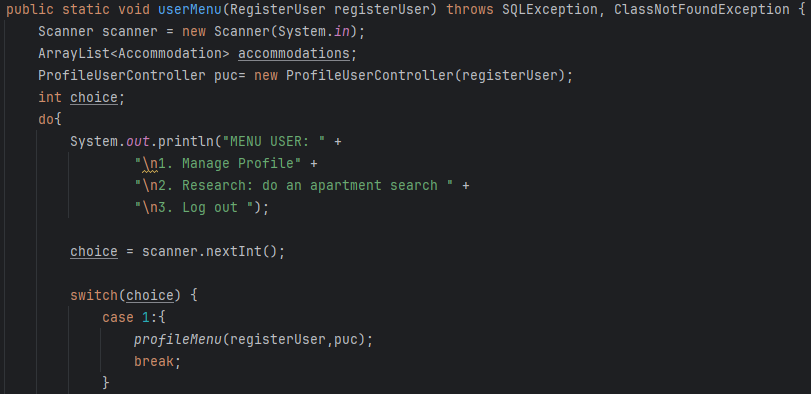
\includegraphics[scale=0.6]{cli/usermenu}
\par\medskip
Figura 16: implementazione del menu dell'utente.
\par\medskip
\end{center} 

\section{Test}

Sono stati realizzati i test per verificare il corretto funzionamento del sistema, focalizzandosi principalmente sulle funzionalità della \textbf{Business Logic} e del \textbf{Dao}. Sono stati realizzati utilizzando la libreria \textbf{JUnit}. 

\subsection{Domain Model Test}

Sono stati implementati i test più rilevanti per il corretto funzionamento della logica di sistema e dei design pattern.
I test implementati sono: 
\begin{itemize}
\item \textbf{AccommodationTest}.
\item \textbf{SearchParametersBuilderTest}.
\end{itemize}

\subsection{Business Logic Test}

Per i controller sono stati effettuati dei test su tutte le loro funzioni (test funzionali), prestando attenzione che seguano le direttive dello \hyperref[usecase]{use case}.
Ne vengono riportati alcuni. 
\begin{itemize}
\item Il test sul metodo di login di un utente che vuole dimostrare che funzioni sia nel caso di flusso normale che alternativo.
\label{test1}
\begin{center}
\hspace*{-0.75cm}
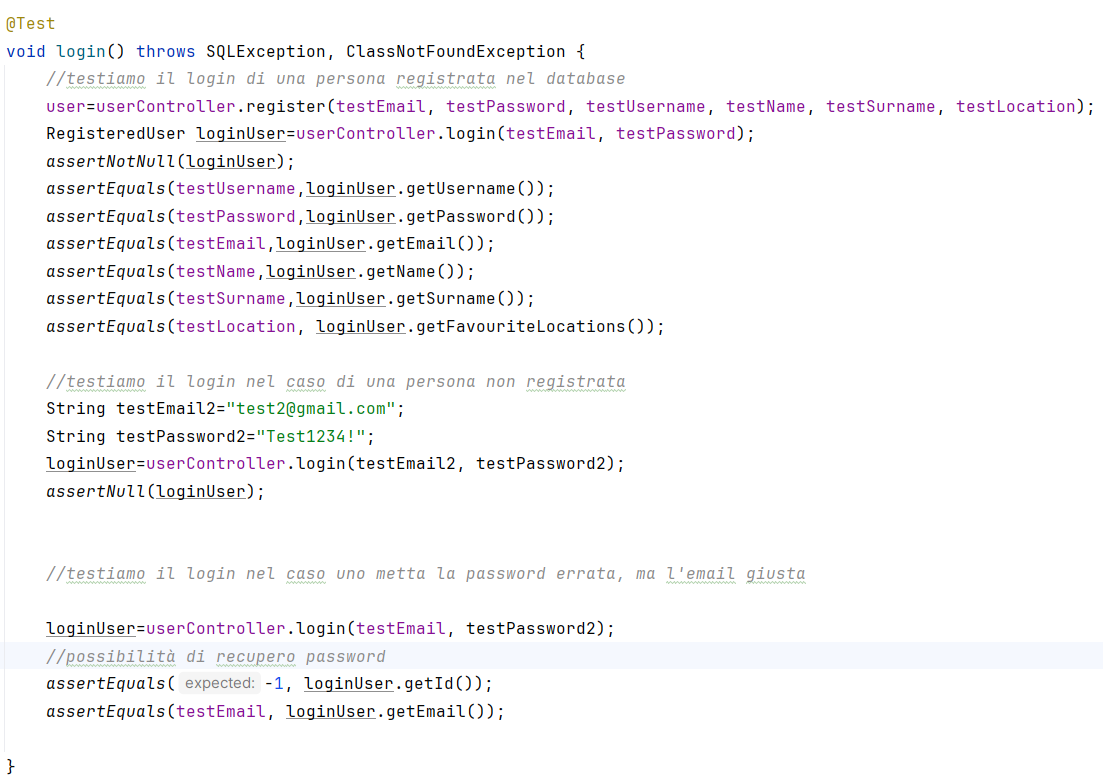
\includegraphics[scale=0.55]{test/BusinessLogic/login}
\par
Figura 17: test che verifica il \hyperref[Usecase1]{login} all'interno dell'applicazione -Tst\#1.
\par   
\end{center}
\label{test2}
\item Il test sulla registrazione da parte di un utente all'applicazione, tenendo conto che funzioni sia nel flusso normale che non.
\begin{center}
\hspace*{-2cm}
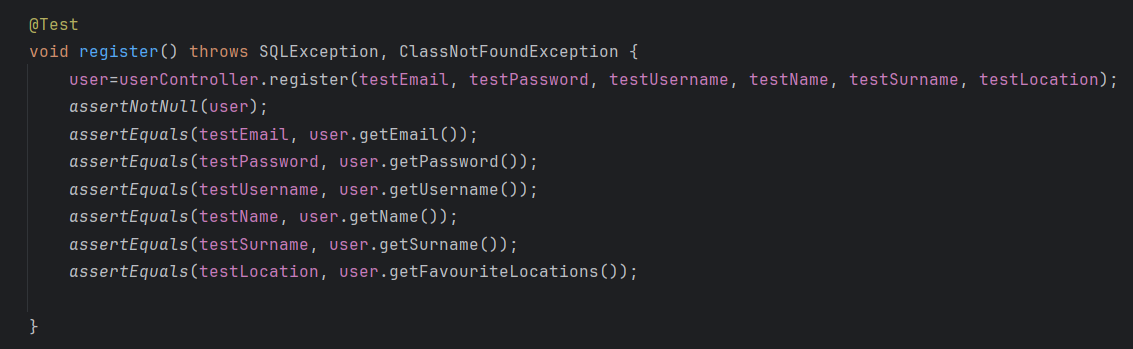
\includegraphics[scale=0.55]{test/BusinessLogic/register}
\par
Figura 18: test che verifica la \hyperref[Usecase4]{registrazione} all'interno dell'applicazione -Tst\#2.
\par\medskip
\end{center}
\end{itemize}
Qui di seguito vengono mostrati tutti i risultati dei test dei metodi della Business Logic:
\par\medskip
\begin{center}
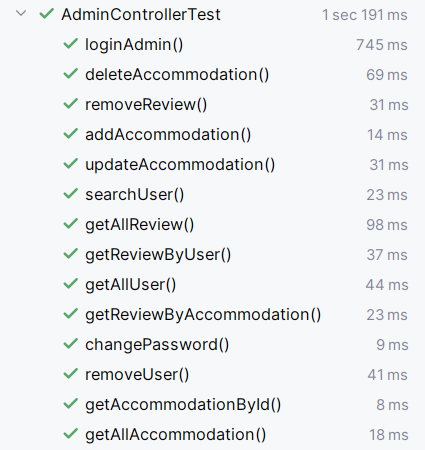
\includegraphics[scale=0.55]{test/BusinessLogic/testAdminController}
\par\medskip
Figura 19: i test per AdminController.
\par\medskip
\end{center}
\begin{center}
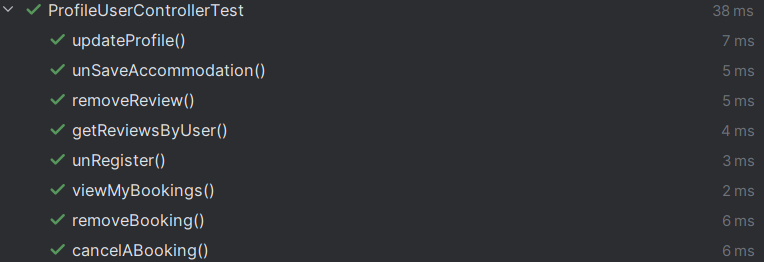
\includegraphics[scale=0.55]{test/BusinessLogic/testProfileUserController}
\par\medskip
Figura 20: i test per ProfileUserController.
\par\medskip
\end{center}



\begin{center}
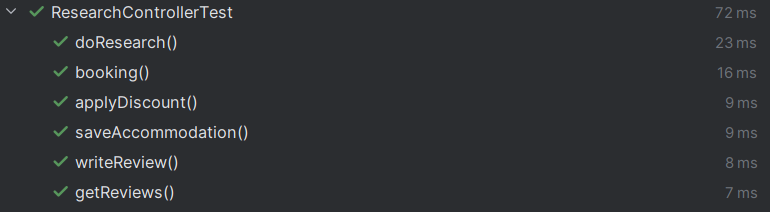
\includegraphics[scale=0.55]{test/BusinessLogic/testResearchController}
\par\medskip
Figura 21: i test per ResearchController.
\par\medskip
\end{center}

\subsection{ORM Test}

Per ogni classe del DAO sono stati effettuati dei test strutturali in modo da assicurarsi che i metodi si relazionino correttamente con il database. Questo controllo viene effettuato attraverso la cattura delle eccezioni in caso di errore.

\subsection{Risultati dei test}
\par\medskip
\begin{center}
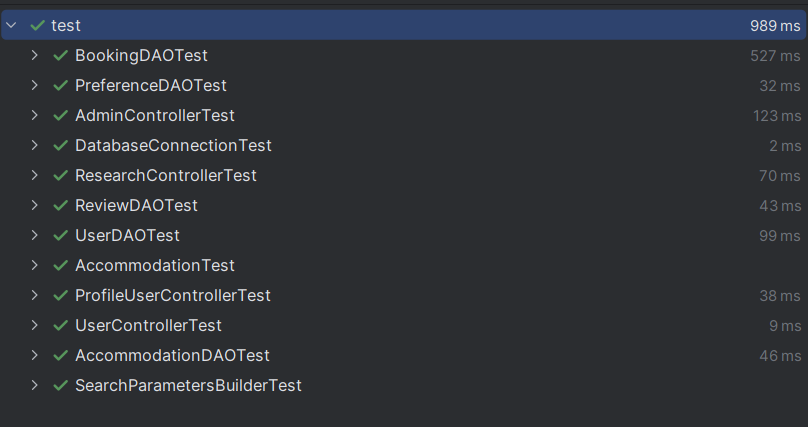
\includegraphics[scale=0.5]{test/BusinessLogic/risultatitest}
\par\medskip
Figura 22: risultati dei test.
\par\medskip
\end{center}


\end{document}
